\documentclass[a4paper,12pt]{article}

\usepackage{graphicx}       % Grafiken einfügen
\usepackage{geometry}       % Seitenränder einstellen
\usepackage{setspace}       % Zeilenabstand
\usepackage{tocloft}        % Inhaltsverzeichnis Formatierung
\usepackage{float}          % Für [H] Platzierung
\usepackage[ngerman]{babel} % Deutsche Einstellungen
\usepackage{booktabs}
\usepackage{fancyhdr}       % Für Kopf- und Fußzeile
\usepackage{lastpage}       % Für Seitenzahl der letzten Seite
\usepackage{comment}
\usepackage{enumitem}
\usepackage{array}
\usepackage{xcolor}
\renewcommand{\arraystretch}{1.5} % Erhöht den Zeilenabstand
\setlength{\arrayrulewidth}{0.5mm} % Dicke der Linien
\setlength{\tabcolsep}{10pt} % Abstand der Spalte


%Keine Ahnung. Irgend a Error wegen Überschrift vo 1.10
\setlength{\headheight}{15pt}
% Den Abstand zwischen Absätzen und Überschriften anpassen
\setlength{\parskip}{0pt} % Abstand zwischen Absätzen
\setlength{\parindent}{0pt} % Kein Einrücken von Absätzen

% Seitenränder
\geometry{a4paper, top=25mm, left=25mm, right=25mm, bottom=35mm} 

% Abstand zwischen Kopfzeile und Text anpassen
\setlength{\headsep}{15mm}  % Abstand zwischen Kopfzeile und Text
\setlength{\footskip}{15mm} % Abstand zwischen Fußzeile und Text 
% Kopf- und Fußzeile definieren
\pagestyle{fancy}
\fancyhf{} % Alle Kopf- und Fußzeilen leeren

% Kopfzeile: Logo links, Kapitelname rechts
%\fancyhead[L]{\includegraphics[width=1.8cm]{Bilder_Sonstiges/Fhooe-logo.png}} % Pfad zum Logo anpassen
\fancyhead[R]{\nouppercase{\leftmark}} % Kapitelname in der Kopfzeile

% Fußzeile: Seitenzahl
\fancyfoot[C]{Seite \thepage\ von\pageref{LastPage}}

% Titelseite ohne Kopf- und Fußzeile
\fancypagestyle{plain}{
  \fancyhf{} % leere Kopf- und Fußzeile
  \fancyfoot[C]{Seite \thepage\ von\pageref{LastPage}} % Seitenzahl zur Titelseite hinzufügen
}  




\begin{document}

% Titelseite
	\begin{titlepage}
		% Hochschullogo
		%\begin{center}
		%	\includegraphics[width=0.4\textwidth]{Bilder_Sonstiges/Fhooe-logo.png} % Pfad zum Logo anpassen
		%\end{center}
		
		% Titel
		\vspace{2cm}
		\begin{center}
			\Huge
			\textbf{Fragenkatalog}
			\vspace{1cm}
			
			\LARGE
			Systems Engineering SYE3IL
		\end{center}
		
		% Ersteller Informationen
		\vspace{3cm}
		\begin{center}
			\Large
			\textbf{Erstellt von:}\\
			Darius Faje \\ Alex\\
			\vspace{2cm}
			Studiengang: MB
		\end{center}
		
		% Ort und Datum
		\vfill
		\begin{center}
			\Large
			13.12.2024
		\end{center}
	\end{titlepage}

\newpage
\tableofcontents % Erstellt das Inhaltsverzeichnis
\newpage

% Teil 1
\section{Teil}

%-------------------------------------------------------------------------------------------
\subsection{Wie kann Komplexität von Systemen charakterisiert werden?}
\textbf{Komplexität} beschreibt, dass das Verhalten eines Modells schwierig zu beschreiben ist, obwohl ausreichend Information über seine Komponenten
 und deren Verflechtungen vorliegen.Was als komplex gilt kommt immer auf die Sichtweise drauf an. $\rightarrow$ Schwer es allgemein zu definieren.
\\

Ein \textbf{komplexes System} ist ein System mit einer großen Zahl and Komponenten und Verknüpfungen, Interaktionen oder Abhängigkeiten, 
welches schwierig beschreibbar, planbar oder steuerbar ist. Test1

\begin{figure}[H]
	\centering
	\includegraphics[width=0.6\linewidth]{Bilder/Teil1_Komplexität.png}
	\caption{Swimlane Diagramm}
\end{figure}

% subsection
%-------------------------------------------------------------------------------------------
\subsection{Nennen Sie externe und interne Komplexitätstreiber!}
	

\begin{table}[h!]
	\centering
	\begin{tabular}{|p{7cm}|p{7cm}|}
		\hline
		\multicolumn{1}{|c|}{\textbf{Externe}} & \multicolumn{1}{c|}{\textbf{Interne}} \\ \hline
		Heterogene Märkte & Aufwendiges Produktkonzept \\ \hline
		Individuelle Kundenbedürfnisse & Hohe Komponentenvielfalt \\ \hline
		Erforderliche Variantenvielfalt & Komplexer Entwicklungsprozess \\ \hline
		Wettbewerb und Gesetzte & Komplexe Fertigung \\ \hline
		Preisdruck & Viele Zulieferer und Projektbeteiligte \\ \hline
	\end{tabular}
	\caption{Vergleich von externen und internen Faktoren}
	\label{tab:extern-intern}
\end{table}
\textbf{Die kann die internen Komplexitätstreiber selber vielleicht beeinflussen die externen nicht!}

% subsection
%-------------------------------------------------------------------------------------------
\subsection{Was versteht man unter Cyber-Physikalischen Systemen}

\begin{itemize}
	\item \textbf{Eine Integration von Computern und physischen Prozessen:}
	\\Physische Prozesse werden durch eingebettete Computer und Netzwerke überwacht, geregelt und gesteuert.
	\item \textbf{Gegenseitige Rückkopplung:} 
	\\Computer und physische Prozesse beeinflussen sich gegenseitig. (Wechselwirkung)
	\item \textbf{Beispiele:} 
	\\Autonome Fahrzeuge, Smartwatch, Produktionsanlagen.
\end{itemize}

% subsection
%-------------------------------------------------------------------------------------------
\subsection{Was versteht man unter Internet of Things}
\begin{itemize}
	\item \textbf{Ein globales Netzwerk von physischen und virtuellen Objekten:} 
	\\Diese Objekte kommunizieren und arbeiten zusammen.
	\item \textbf{Technologie zur Unterstützung des Menschen:}
	\\Ermöglicht Interaktion zwischen Mensch und vernetzten Systemen sowie zwischen den Systemen selbst.
	\item \textbf{Beispiele:} 
	\\Kühlschränke mit automatischer Nachbestellung. Hat sich besonders bei Supermärkten durchgesetzt
\end{itemize}


% subsection
%-------------------------------------------------------------------------------------------
\subsection{Was versteht man unter Systems of Systems?}
Ein Systems of Systems (SoS) ist:
\begin{itemize}
	\item \textbf{Ein Verbund autonomer Systeme:} 
	\\Diese Systeme arbeiten zusammen, um ein neues, komplexeres System mit zusätzlicher Funktionalität zu schaffen.
	
	\item \textbf{Charakteristische Merkmale:}
	\begin{itemize}
		\item \textbf{Operative Unabhängigkeit der Subsysteme:} Jedes Subsystem arbeitet unabhängig.
		\item \textbf{Unabhängige Verwaltung der einzelnen Systeme:} Die Systeme werden eigenständig verwaltet.
		\item \textbf{Evolutionäre Entwicklung:} Ständige Weiterentwicklung und Anpassung der Systeme/Komponenten. (ohne das das gesamt System zusammenbricht)
		\item \textbf{Emergentes Verhalten:} Ausfall von einem Teil führt nicht zum Ausfall des gesamten Systems.
		\item \textbf{Geografische Verteilung der Systeme:} Die Systeme können an verschiedenen geografischen Orten verteilt sein.
	\end{itemize}
\end{itemize}


% subsection
%-------------------------------------------------------------------------------------------
\subsection{Was ist ein Produkt-Service-System (PSS)? }
Ist ein \textbf{Leistungsangebot} mit signifikanten \textbf{Anteilen an Sachgütern als auch Dienstleistungen}. Dienstleistungen sind integraler Bestandteil des PSS. 

Z.B. Carsharing, Leasing

% subsection
%-------------------------------------------------------------------------------------------
\subsection{Welche Klassen von Produkt-Service-Systemen gibt es?}
Einteilung in 3 Teile:
\begin{itemize}
    \item \textbf{Reines Produkt}
        \begin{itemize}
            \item Produkt im Besitz des Kunden.
            \item Kunde selber verantwortlich.
            \item z.B. Kauf Waschmaschine, Auto
        \end{itemize}
    \item \textbf{Reiner Service}
        \begin{itemize}
            \item Reine Dienstleistung.
            \item Produkt nicht im Besitz des Kunden.
            \item z.B. Waschsalon, Beratung
        \end{itemize}

    \item \textbf{Produkt Service Systeme:}
    
    \begin{itemize}
    	\item \textbf{Produktorientiert:}
    	\begin{itemize}
    		\item Klassischer Verkauf im Vordergrund.
    		\item Produktbezogen, Beratung (Auto + Einschulung oder Wartung)
    	\end{itemize}
    	
    	\item \textbf{Nutzungsorientiert:}
    	\begin{itemize}
    		\item Nutzung des Produktes im Vordergrund.
    		\item Produkt im Besitz des Anbieters.
    		\item z.B. Leasing, Mieten, Pooling
    	\end{itemize}
    	
    	\item \textbf{Ergebnisorientiert:}
        \begin{itemize}
        	\item Ergebnis steht im Vordergrund
			\item Übereinkunft zwischen Anbieter und Kunde über zu erreichendes Ziel.
			\item Die Wahl des Produktes und des Vorgehens obliegt dem Anbieter.
			\item Honorar nach Ergebnis
		\end{itemize}
    	
    \end{itemize}
        
\end{itemize}

% subsection
%-------------------------------------------------------------------------------------------
\subsection{Aus welchen Bestandteilen besteht ein System?}

\begin{figure}[H]
	\centering
	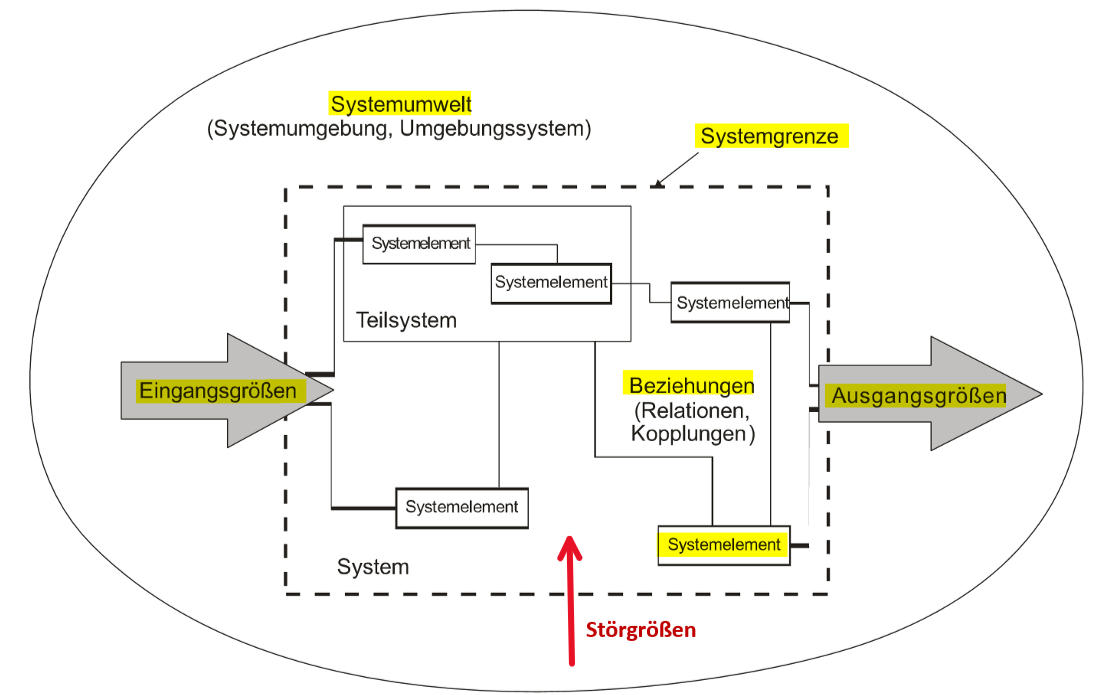
\includegraphics[width=0.7\linewidth]{Bilder/Teil1_zentraleDarstellungSystem.png}
	\caption{Swimlane Diagramm}
\end{figure}

\begin{itemize}
    \item \textbf{Systemumwelt}
    \begin{itemize}
        \item Alles, was nicht in das System einbezogen ist (abgetrennt an Systemgrenze).
    \end{itemize}
    
    \item \textbf{Stoff-, Energie-, Informationsfluss}
    \begin{itemize}
        \item Art und Weise der Interaktion mit Systemumwelt.
        \item Systemgrenze so wählen, dass Kopplung zur Umgebung sehr viel schwächer als Kopplung im Inneren ist.
    \end{itemize}
    
    \item \textbf{Eingang}
    \begin{itemize}
        \item Stellt Relation der Umwelt zum System dar.
        \item Vom Verhalten des Systems nicht beeinflusst.
        \item \textbf{Stellgrößen}: gezielte Veränderung des Eingangs.
        \item \textbf{Störgrößen}: unkontrollierte Veränderung des Eingangs (z.B. Rauschen).
    \end{itemize}
    
    \item \textbf{Ausgang}
    \begin{itemize}
        \item Stellt Relation vom System zur Umgebung dar (z.B. Messgröße).
    \end{itemize}
    
    \item \textbf{Teilsystem}
    \begin{itemize}
        \item Element eines Systems, welches weitere Elemente enthält (enthält eigenes System - Subsystem).
    \end{itemize}
    
        \item \textbf{Störgrößen}
    \begin{itemize}
    	\item Nicht gewünschte Eingangsgrößen (Bsp. Rauschen)
    \end{itemize}
    
\end{itemize}

% subsection
%-------------------------------------------------------------------------------------------
\subsection{Begriffe wofür Systems Engineering steht!}
\begin{itemize}[itemsep=0pt, topsep=10pt]
    \item Interdisziplinär
    \item Früh (in Entwicklungsprozess)
    \item Dokumentieren (Anforderungen)
    \item Gesamtheitlich (auf System Bezogen)
    \item Wirtschaftlich (Bedürfnisse des Kunden)
    \item Technisch
\end{itemize}

% subsection
%-------------------------------------------------------------------------------------------
\subsection{Was bedeutet SADT + Beispiel.}
\textbf{SADT = Structured Analysis and Design Technique}

Beschreibt Aktivitäten und Informationsflüsse. z.B. Bauteilbearbeitung

\begin{figure}[H]
    \centering
    \begin{minipage}[t]{0.45\textwidth}  % 't' sorgt dafür, dass die minipage an der Oberkante ausgerichtet ist
        \centering
        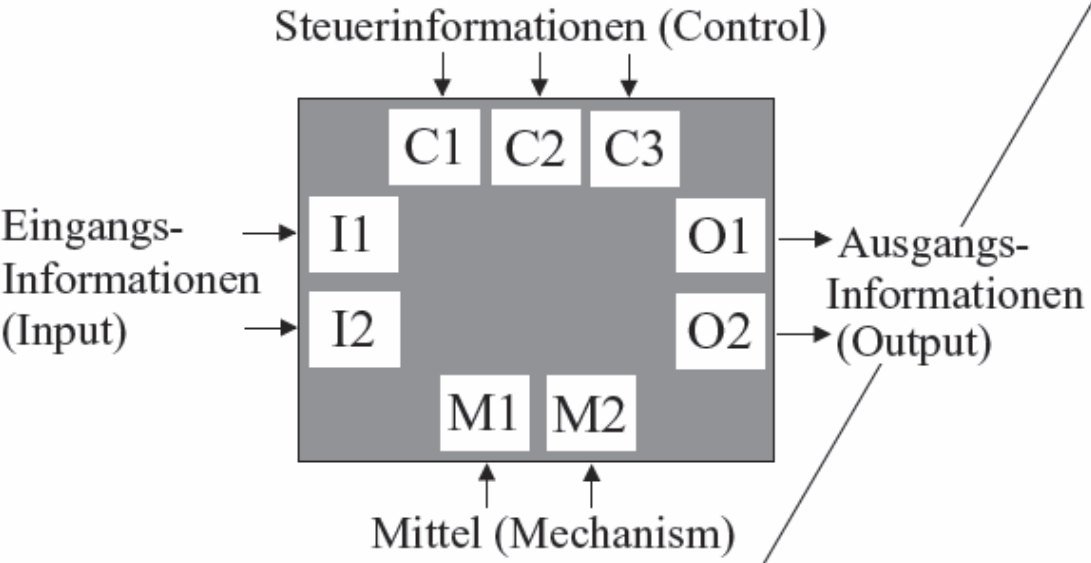
\includegraphics[width=\linewidth]{Bilder/Teil1_SADT_Allgemein.png} % Bild 1
        \caption{SADT Allgemein}
    \end{minipage} \hfill
    \begin{minipage}[t]{0.45\textwidth}  % 't' sorgt für gleiche Ausrichtung der Unterschriften
        \centering
        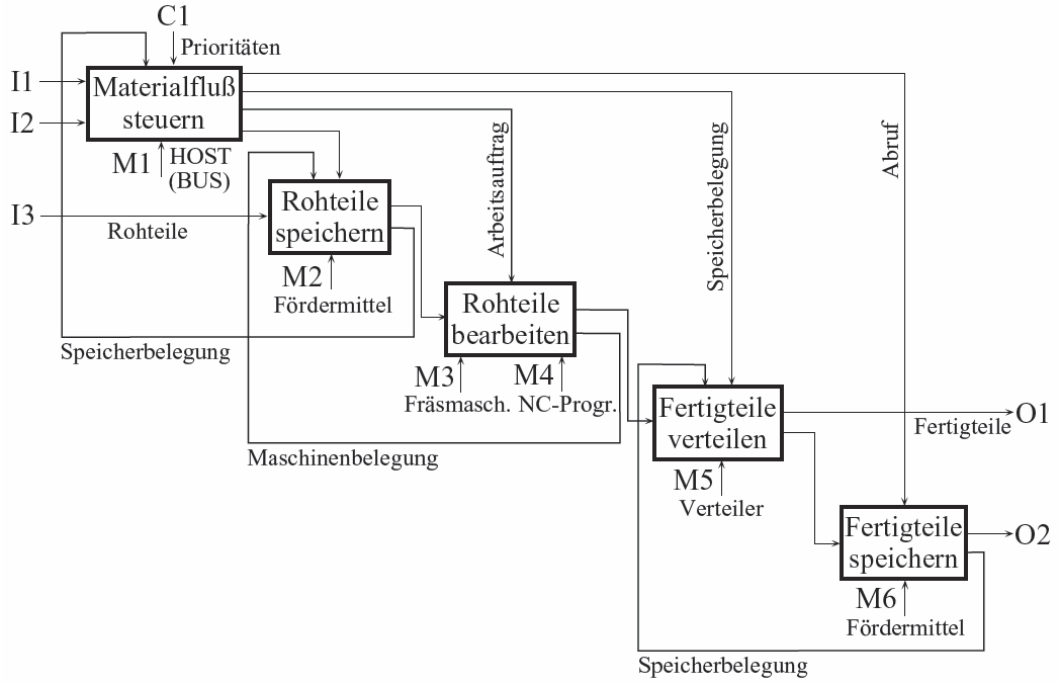
\includegraphics[width=\linewidth]{Bilder/Teil1_SADT_Beispiel.png} % Bild 2
        \caption{SADT Praxisbeispiel}
    \end{minipage}
    %\caption{Structured Analysis and Design Technique - SADT}
\end{figure}




% subsection
%-------------------------------------------------------------------------------------------
\subsection{Was sind Swimlane-Diagramme + Beispiel}
Sind eine Art von \textbf{Flussdiagrammen}, welche zeigen wer in einem Prozess zuständig ist.

\textbf{Verantwortungsbereiche = Swimlanes}

\begin{figure}[H]
    \centering
    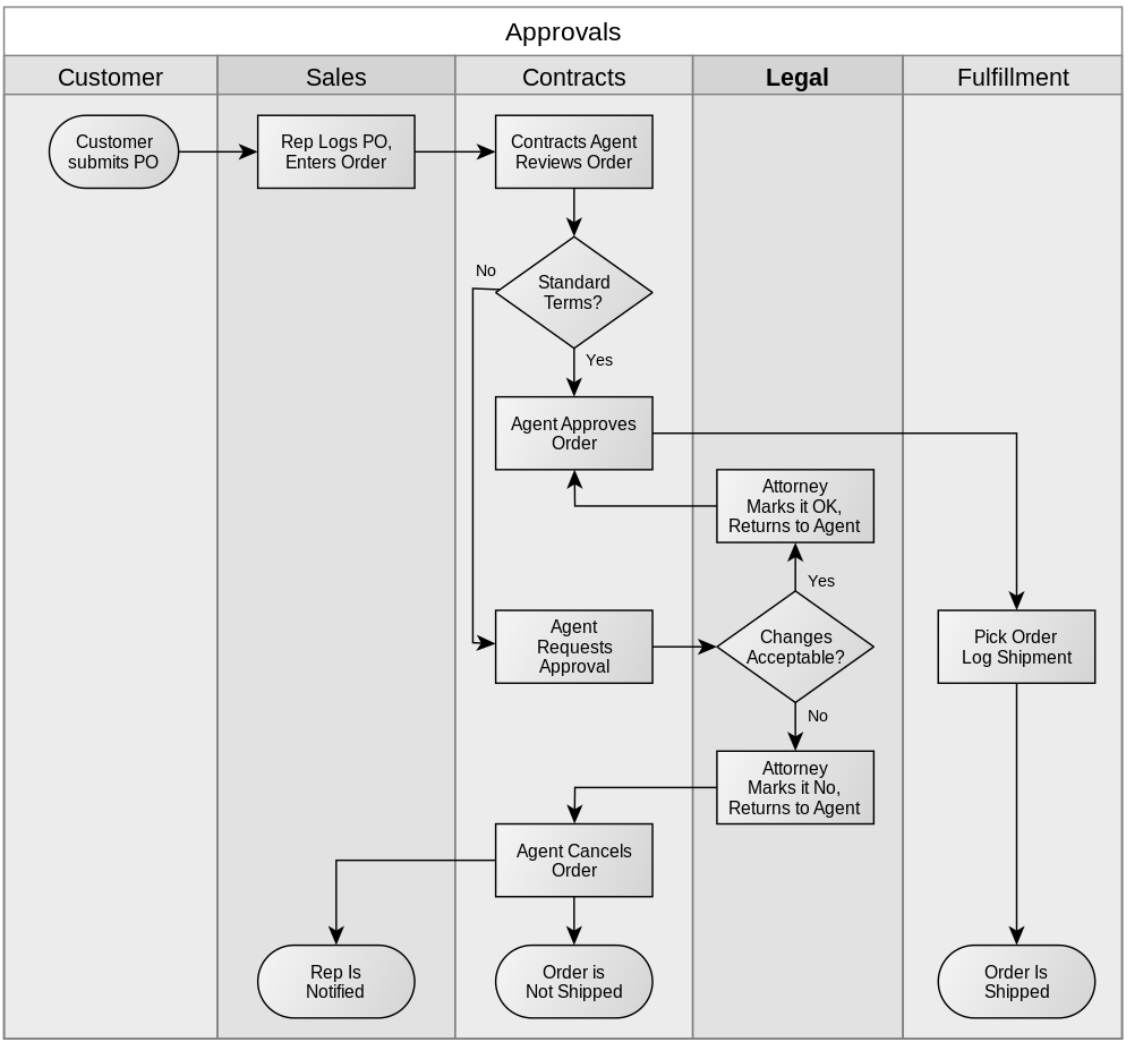
\includegraphics[width=0.7\linewidth]{Bilder/Teil1_SwimlaneDiagramm.png}
    \caption{Swimlane Diagramm}
\end{figure}

% subsection
%-------------------------------------------------------------------------------------------
\subsection{Vier Grundregeln des Agilen Manifests}

\textbf{Grundlagen - Theoretisch}
\begin{itemize}
    \item Individuen und Interaktionen haben Vorrang zu Prozessen und Werkzeugen
    \item Funktionsfähige Produkte haben Vorrang zu ausgedehnter Dokumentation
    \item Zusammenarbeit mit Kunden hat Vorrang vor Vertragshandlungen
    \item Reagieren auf Änderungen hat Vorrang vor strikter Planverfolgung
\end{itemize}

\textbf{Grundlagen - Praxisbeispiele}
\begin{itemize}
    \item Arbeiten im Team
    \item Fokus auf technische Aufgabenstellung
    \item Denke an Kunden
    \item Flexibel für Änderungen
\end{itemize}

% subsection
%-------------------------------------------------------------------------------------------
\subsection{Bedeutung SCRUM + Rollen  }
\textbf{SCRUM = Vorgehensmodell der agilen Softwareentwicklung.}

Geht davon aus, dass Entwicklungen aufgrund ihrer Komplexität nicht im Vorraus detailliert planbar sind.

\textbf{Stärken:} überschaubares Rahmenwerk mit wenig Rollen, Artefakten und Ereignissen.

\textbf{Rollen}
\begin{itemize}
    \item Product Owner
    \begin{itemize}
        \item Für wirtschaftlichen Erfolg des Produktes verantwortlich.
        \item Vertritt Kundeninteressen. Sind aber nicht identisch.
    \end{itemize}
    
    \item Entwickler Team
    \begin{itemize}
        \item Keine hierarchischen Strukturen.
        \item Setzt Anforderungen von Product Owner um.
    \end{itemize}
    
    \item Scrum Master
    \begin{itemize}
        \item Moderiert alle Ereignisse und sorgt für störungsfreies Arbeiten.
        \item Kein Teammitglied und nicht weisungsbefugt.
        \item Stellt Einhaltung von Scrum-Regeln sicher.
    \end{itemize}
    
\end{itemize}


% Teil 2
\section{Teil}
beinhaltet folgende Foliensätze:

\begin{itemize}
    \item Teil 2: Systemanforderungen (Requirements Engineering)

\end{itemize}

% subsection
%-------------------------------------------------------------------------------------------
\subsection{Was versteht man unter einem Requirement?}

Ein \textbf{Requirement} definiert geforderte oder gewünschte Eigenschaften.

Betrifft \textbf{Funktionalität}, ein \textbf{Qualitätsmerkmal}, eine \textbf{Bedingung} oder \textbf{Fähigkeit}.

% subsection
%-------------------------------------------------------------------------------------------
\subsection{Was ist ein Stakeholder?}

Ist eine \textbf{Person} oder \textbf{Organisation}, welche Einfluss (direkt oder indirekt) auf die Anforderungen des Systems hat.

% subsection
%-------------------------------------------------------------------------------------------
\subsection{Wie kann man Requirements Engineering und Requirements Management unterscheiden?}

\textbf{Requirements Engineering}

\begin{itemize}
    \item Entwickeln der Anforderungsbasis.
    \item Analysieren, Ermitteln, Strukturieren, Spezifizieren von Anforderungen.
\end{itemize}

\textbf{Requirements Management}
\begin{itemize}
    \item Arbeiten mit Anforderungen.
    \item Dokumentieren, Ändern, Rückverfolgen, Versionieren von Anforderungen.
\end{itemize}

% subsection
%-------------------------------------------------------------------------------------------
\subsection{Wie werden Anforderungen angegeben?   ---nicht sicher---}

\textbf{Anforderung}
\begin{itemize}
    \item Geforderte Eigenschaft bezogen auf Produkt oder Entwicklung.
    \item Formal durch Merkmale und Ausprägungen ausdrücken.
    \item Repräsentiert ein Entwicklungsziel.
\end{itemize}

\textbf{Merkmal}
\begin{itemize}
    \item Beschreibt Bezugsobjekt der Anforderung (z.B. Namen).
\end{itemize}

\textbf{Ausprägung}
\begin{itemize}
    \item Bezeichnet den Sollwert für das Anforderungsmerkmal.
    \item Beinhaltet bei quantitativen Anforderungen einen Wertebereich und Einheit.
    \item Beinhaltet bei qualitativen Anforderungen einen verbalen Ausdruck.
\end{itemize}

\begin{figure}[H]
    \centering
    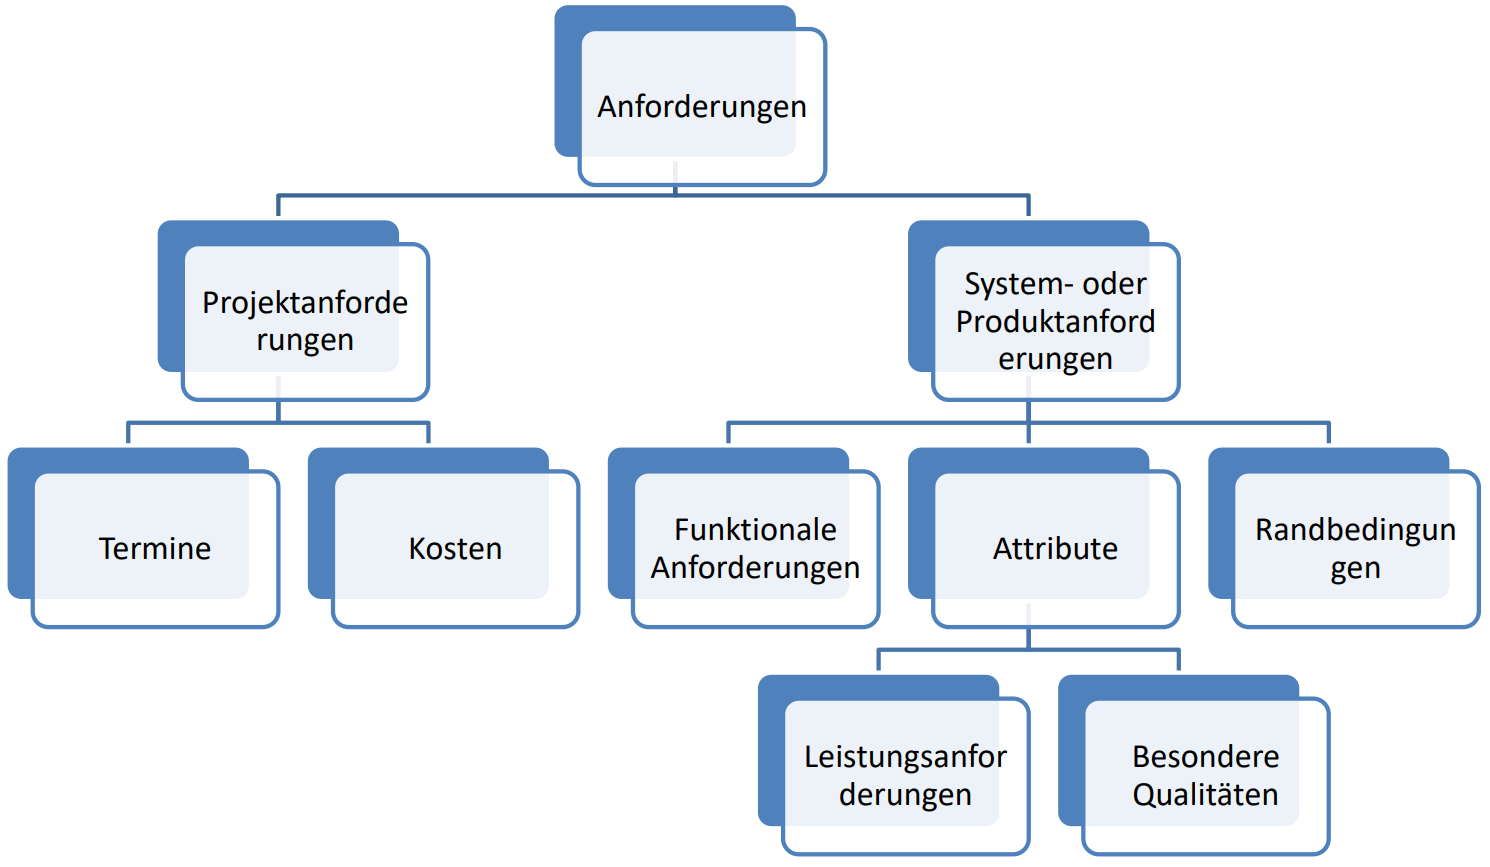
\includegraphics[width=0.7\linewidth]{Bilder/Teil2_KlassifikationAnforderungen.png}
    \caption{Klassifikation von Anforderungen}
\end{figure}

% subsection
%-------------------------------------------------------------------------------------------
\subsection{Nennen Sie Funktionale Anforderungen. (Zusatz!)}

Beschreiben funktionale Aspekte des Systems.

\begin{itemize}
    \item Fragestellung: \textbf{Was tut das System}
    \item Beschreibt Funktionen, Eingaben, Ausgaben (Daten, Fehlermeldungen, ...) des Systems.
    \item Beschreiben wichtige Systemzustände und das Verhalten des Systems.
    \item Bsp.: Der Alarm soll ausgelöst werden, sobald der Sensor das Zerbechen der Fensterscheibe detektiert.
\end{itemize}

% subsection
%-------------------------------------------------------------------------------------------
\subsection{Nennen Sie Nicht-Funktionale Anforderungen.}

\begin{itemize}
    \item \textbf{Technologische Anforderungen}
        \begin{itemize}
            \item schränken Lösungsraum des Systems ein.
            \item Definieren vorgegebene Lösungswege.
        \end{itemize}
    \item \textbf{Qualitätsanforderungen}
        \begin{itemize}
            \item Definieren die Qualität des Produktes.
        \end{itemize}
    \item \textbf{Anforderungen an Benutzeroberfläche}
        \begin{itemize}
            \item Anforderungen an die Bedienung des Produktes.
        \end{itemize}
    \item \textbf{Nebenprodukte}
        \begin{itemize}
            \item Notwendig für Funktion bzw. Verständnis des Produktes (z.B. Doku).
            \item Unterpunkt2
        \end{itemize}
    \item \textbf{Anforderungen an durchzuführende Tätigkeiten}
        \begin{itemize}
            \item Tätigkeiten, welche nach dem Entwicklungsprozess anfallen (z.B. Wartung)
        \end{itemize}
    \item \textbf{Rechtlich- Vertragliche Anforderungen}
        \begin{itemize}
            \item Anforderungen zwischen Vertragspartnern vor Entwicklungsbeginn.
        \end{itemize}
\end{itemize}


% subsection
%-------------------------------------------------------------------------------------------
\subsection{Was sind typischen Schritte im Requirements Engineering?}

\begin{itemize}
    \item Anforderungen \textbf{erheben} (z.B. Befragung von Stakeholdern)
    \item Anforderungen \textbf{dokumentieren} (z.B. Lastenheft)
    \item Anforderungen \textbf{verifizieren} (z.B. Hinblick auf Spezifikation)
    \item Anforderungen \textbf{validieren} (z.B. Hinblick auf Zweck oder Anforderungen)
    \item Anforderungen \textbf{verwalten} (z.B. Administrative Werkzeuge wie: Freigeben, Ändern, Rückverfolgen)
\end{itemize}

% subsection
%-------------------------------------------------------------------------------------------
\subsection{Nennen Sie Quellen für Anforderungen?}

\textbf{3 Teilbereiche zur Gewinnung von Anforderungen}
\begin{itemize}
    \item Identifizierung relevanter Anforderungsquellen
    \item Gewinnung von existierenden Anforderungen
    \item Entwicklung von innovativen Anforderungen
\end{itemize}

\textbf{Methoden}
\begin{itemize}
    \item Interviews
    \item Workshops
    \item Beobachtungen
    \item Schriftliche Befragung
    \item Perspektivenbasiertes Lesen
\end{itemize}

\begin{figure}[H]
    \centering
    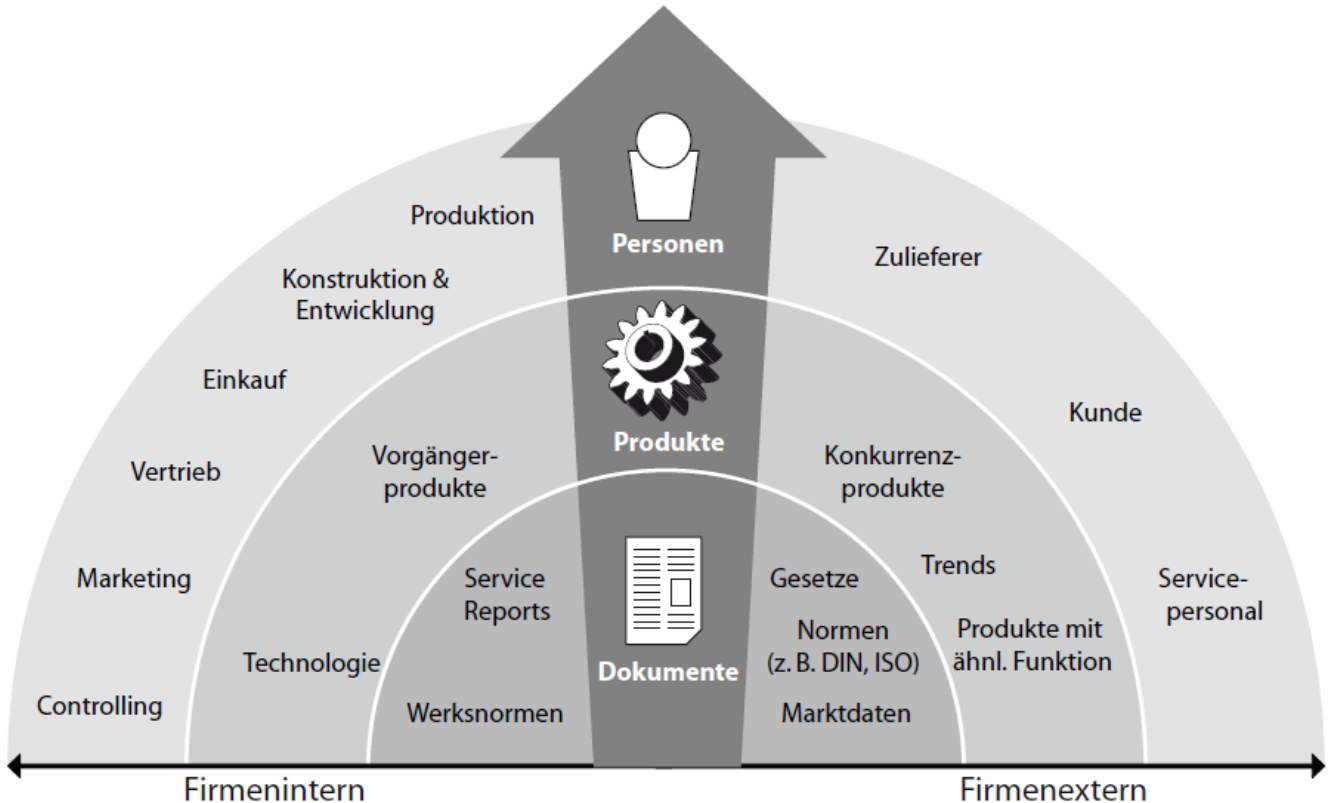
\includegraphics[width=0.7\linewidth]{Bilder/Teil2_QuellenAnforderungen.png}
    \caption{Klassifikation von Anforderungen}
\end{figure}

% subsection
%-------------------------------------------------------------------------------------------
\subsection{Was sind Qualitätskriterien für Anforderungen?}

\textbf{Smarte Anforderungen}
\begin{itemize}
    \item Spezifiziert
    \item Messbar
    \item Akzeptiert
    \item Realisierbar
    \item Terminiert
    \item Eindeutig
    \item Vollständig
    \item Bewertet
\end{itemize}

% subsection
%-------------------------------------------------------------------------------------------
\subsection{Was sind typische Bestandteile einer Anforderungsliste?}

\textbf{Inhalte der Anforderungsliste}
\begin{itemize}
    \item Forderungen
        \begin{itemize}
            \item Müssen erfüllt werden.
            \item Können auch als Mindset oder Maximalforderungen definiert.
        \end{itemize}
    \item Wünsche
        \begin{itemize}
            \item Sollen erfüllt werden.
            \item Aufgabenlösung auch ohne Erfüllung der Wünsche.
        \end{itemize}
    \item Quantitative Angaben
        \begin{itemize}
            \item Forderungen und Wünsche so weit wie möglich mit konkreten Werten angeben (Eindeutige Interpretation).
        \end{itemize}
    \item Qualitative Angaben
        \begin{itemize}
            \item Besondere Anforderungen oft ohne definierte Werte angegeben.
        \end{itemize}
    \item Administrative und ordnenden Angaben
        \begin{itemize}
            \item Benutzer
            \item Projektbezeichnung
            \item relevante Datum
            \item Ersteller
            \item Änderer
        \end{itemize}
\end{itemize}

% subsection
%-------------------------------------------------------------------------------------------
\subsection{Mit welcher Methode können Zielkonflikte erkannt werden und erklären Sie diese! }



\textbf{Methode : Korrelationsmatrix} \\

\textbf{Gründe für Korrelationsmatrix}
\begin{itemize}
    \item Bereinigung der Anforderungsliste um Inkonsistenzen und Redundanzen.
    \item Analyse von Wechselbeziehungen zwischen Anforderungen und Identifikation von Zielkonflikten.
    \item Priorisierung von Anforderungen.
\end{itemize}


\begin{itemize}
    \item Wechselbeziehung zwischen Anforderungen eintragen.
    \item Gewichtung zur Darstellung der Stärke der Abhängigkeit .
    \item Matrix oft symmetrisch.
\end{itemize}

\begin{figure}[H]
    \centering
    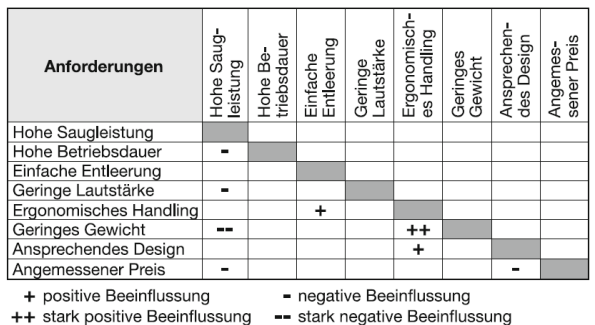
\includegraphics[width=0.7\linewidth]{Bilder/Teil2_Korrelationsmatrix_Beispiel.png}
    \caption{Beispiel Korrelationsmatrix}
\end{figure}

% Teil 3
\section{Teil}
beinhaltet folgende Foliensätze:

\begin{itemize}
    \item Teil 3a:  Produktarchitektur, Modularisierung
    \item Teil 3b:  Design Structure Matrix

\end{itemize}

% subsection
%-------------------------------------------------------------------------------------------
\subsection{Welche drei Schritte sind zur Bildung einer Modularen Produktarchitektur relevant?}

\begin{itemize}
    \item \textbf{Identifikation der Komponenten}
        \begin{itemize}
            \item Produkt in Komponenten zerlegt, um Module zu bilden.
            \item Granularität beschreibt den Grad der Zerlegung.
            \item Granularität muss zu Komplexität und Zielen passen.
        \end{itemize}
    \item \textbf{Analyses der Abhängigkeiten von Komponenten}
        \begin{itemize}
            \item Interaktionen oder Abhängigkeiten der Komponenten untereinander analysieren.
            \item z.B.: Mechanische Schnittstellen mit modularer Bauweise - mechanische Interaktion der Komponenten analysieren.
        \end{itemize}
    \item \textbf{Gruppierung zu Modulen}
        \begin{itemize}
            \item Komponenten zu Module zusammenfassen.
        \end{itemize}
\end{itemize}

% subsection
%-------------------------------------------------------------------------------------------
\subsection{Welche Funktions- und Bausteinarten in Baukästen kennen Sie?}

\begin{itemize}
    \item \textbf{Grundfunktionen}
        \begin{itemize}
            \item Grundlegende, immer wiederkehrende Funktionen.
            \item Mit anderen Grundfunktionen zur Bildung der Gesamtfunktion.
        \end{itemize}
    \item \textbf{Hilfsfunktionen}
        \begin{itemize}
            \item Funktion Verbinden und Anschließen.
            \item Kopplung zwischen Funktionsbausteinen. 
        \end{itemize}
    \item \textbf{Sonderfunktionen}
        \begin{itemize}
            \item Spezielle, ergänzende oder spezifische Teilfunktionen zu Bildung der Gesamtfunktion.
        \end{itemize}
    \item \textbf{Anpassungsfunktionen}
        \begin{itemize}
            \item Schnittstelle zur Umwelt mit anderen Systemen. 
            \item Auftragsspezifisch anzupassen.
            \item System wird mechanisch, elektrisch und informationstechnisch mit Umwelt verbunden.
        \end{itemize}
    \item \textbf{Auftragsspezifische Funktionen}
        \begin{itemize}
            \item Für projektspezifische Funktionen, welche nicht standardmäßig angeboten werden.
        \end{itemize}
    \item \textbf{MUSS – Funktionen}
        \begin{itemize}
            \item Umfassen Grund-, Hilfs-, und Anpassungsfunktionen. 
            \item Zwingend notwendig zur Bildung der Gesamtfunktion. 
        \end{itemize}
    \item \textbf{KANN – Funktionen}
        \begin{itemize}
            \item Aus Sonderfunktionen gebildet.
            \item Nice to Have-Elemente.
        \end{itemize}
\end{itemize}


% subsection
%-------------------------------------------------------------------------------------------
\subsection{Was sind Vor- und Nachteile von Produktplattformen?}

\textbf{Vorteile}
\begin{itemize}
    \item Einfache Erstellung von Varianten. Anpassung an geänderte Varianten.
    \item Abdeckung weiterer Marktsegmente bei geringem Aufwand.
    \item Komponenten trotzdem in großen Stückzahlen produzierbar (Kostenvorteil).
\end{itemize}

\textbf{Nachteile}
\begin{itemize}
    \item Zusätzlicher Aufwand für die Verwaltung der Varianten.
    \item Hoher Planungsaufwand zu Beginn.
\end{itemize}

% subsection
%-------------------------------------------------------------------------------------------
\subsection{Was versteht man unter Kundenindividuelle Massenproduktion?}

Kompromiss aus Massenfertigung und individueller Anpassung. Massenproduktion ist effizient, aber nicht auf Kundenwunsch anpassbar. Einsatz von Produktplattformen. 

z.B. Autoindustrie: Selbes Modell in vielen unterschiedlichen Varianten (Farbe, Ausstattung, ...).


% subsection
%-------------------------------------------------------------------------------------------
\subsection{Was ist ein Graph und welche Arten gibt es?}

\begin{itemize}
    \item Mathematische Grundlage zur Darstellung eines beliebigen Netzwerks.
    \item Ursprung: Königsberger Brückenproblem.
    \item Zur generischen Beschreibung von Netzwerken.
    
    \begin{figure}[H]
        \centering
        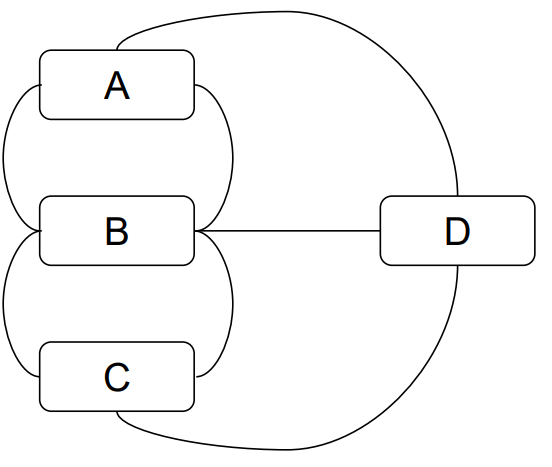
\includegraphics[width=0.6\linewidth]{Bilder/Teil3_Graph_Allgemein.png}
        \caption{Graph allgemein}
    \end{figure}

    \item \textbf{Eigenschaften:}
        \begin{itemize}
            \item Gerichtet, Ungerichtet oder beides
            \item Knoten als auch Kanten können gewichtet sein.
            \item Kante kann zu Ursprungsknoten führen.
            \item Keine, eine oder mehrere Kanten können zwei Knoten verbinden.
            \item Offene oder lose Enden.
        \end{itemize}
    \item \textbf{Charakteristiken:}
        \begin{itemize}
            \item Unterscheidung Knoten und Kanten.
            \item Zwei Kanten angrenzend, wenn sie sich einen Knoten teilen.
            \item Knoten aneinander angrenzend, wenn sie sich eine Kante teilen.
            \item Eine Kante kann zu einem Knoten führen oder weggehen.
            \item Anzahl der Kanten zu einem Knoten bestimmt dessen Ordnung.
        \end{itemize}
    \item \textbf{Arten von Graphen:}
        \begin{itemize}
            \item Ungerichtet, Gerichtet, Beides
            \begin{figure}[H]
                \centering
                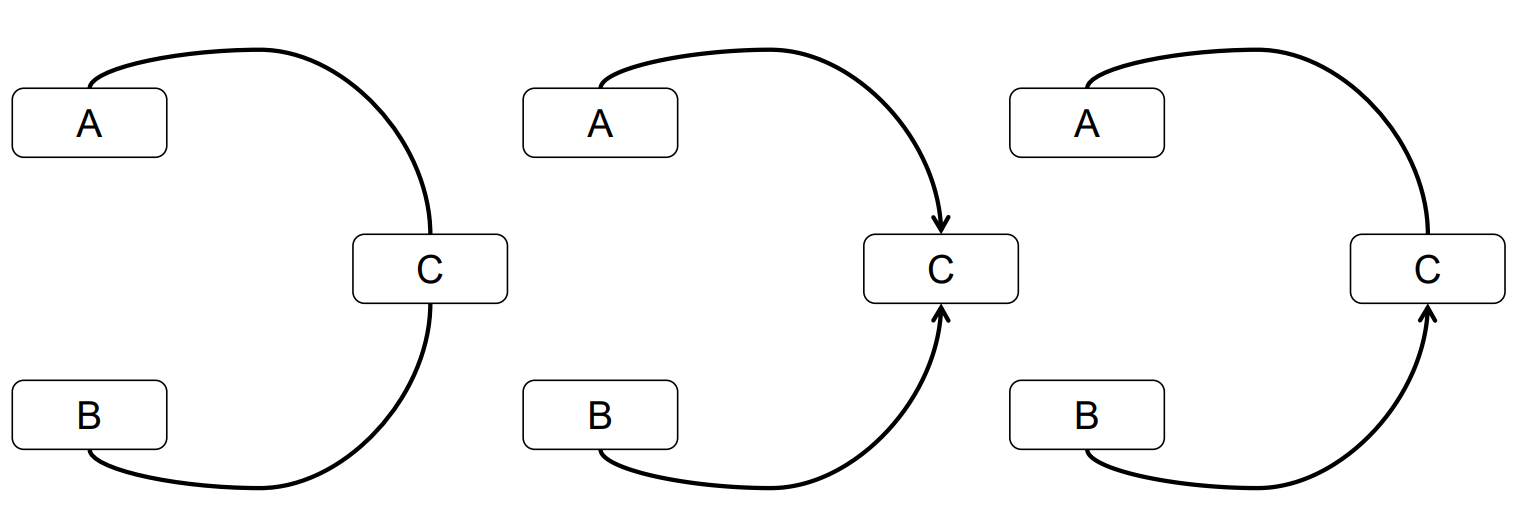
\includegraphics[width=0.7\linewidth]{Bilder/Teil3_ArtenGraphen.png}
                \caption{Arten von Graphen}
            \end{figure}
        \end{itemize}
\end{itemize}


% subsection
%-------------------------------------------------------------------------------------------
\subsection{Erklären Sie einen gewichteten Graphen?}
Ein Gewichteter Graph hat \textbf{Gewichtungsfaktoren} für die Knoten und Kanten.

z.B. Kosten, Bearbeitungs- und Transportzeit

\begin{figure}[H]
    \centering
    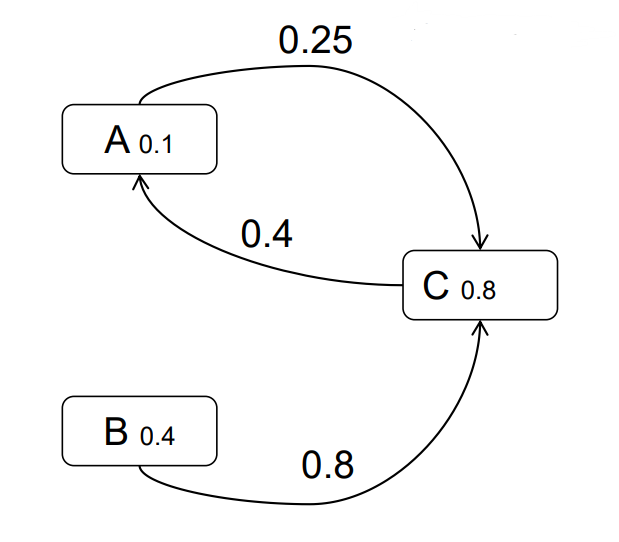
\includegraphics[width=0.6\linewidth]{Bilder/Teil3_GewichteterGraph.png}
    \caption{Beispiel Gewichteter Graph}
\end{figure}


% subsection
%-------------------------------------------------------------------------------------------
\subsection{Wofür steht der Begriff DSM?}
\textbf{Design Structure Matrix}
\begin{itemize}
    \item Zeigt Verbindungen zwischen Systemelementen in Matrixform.
    \item Elemente (z.B. Aktivitäten eines Prozesses) in Zeilen und Spalten einer symmetrischen Matrix anhand logischer Abhängigkeiten aufgetragen. 
    \item Leserichtung aufgetragen: \textbf{Zeile beeinflusst Spalte}
    \item Diagonale bleibt unbeachtet.
    \item DSM innerhalb einer Domäne modellieren, um Aussagefähigkeit zu gewähleisten.
    \item \textbf{Vorteile:}
        \begin{itemize}
            \item Einfache und präzise Möglichkeit komplizierte Systeme darzustellen.
            \item Erlaubt Einsatz von leistungsfähigen Analysemöglichkeiten (Clustering, Sequenzierung, Matrixanalysen).
        \end{itemize}
    \item \textbf{Nachteile:}
        \begin{itemize}
            \item Knoten referenzieren nicht auf Kanten.
            \item Eigenschaften der Kanten können nur bedingt dargestellt werden.
            \item Zeitliche Änderungen der Struktur schwierig darzustellen.
            \item Schwierig zu managen bei hierarchischer Aufteilung.
        \end{itemize}
\end{itemize}

\begin{figure}[H]
    \centering
    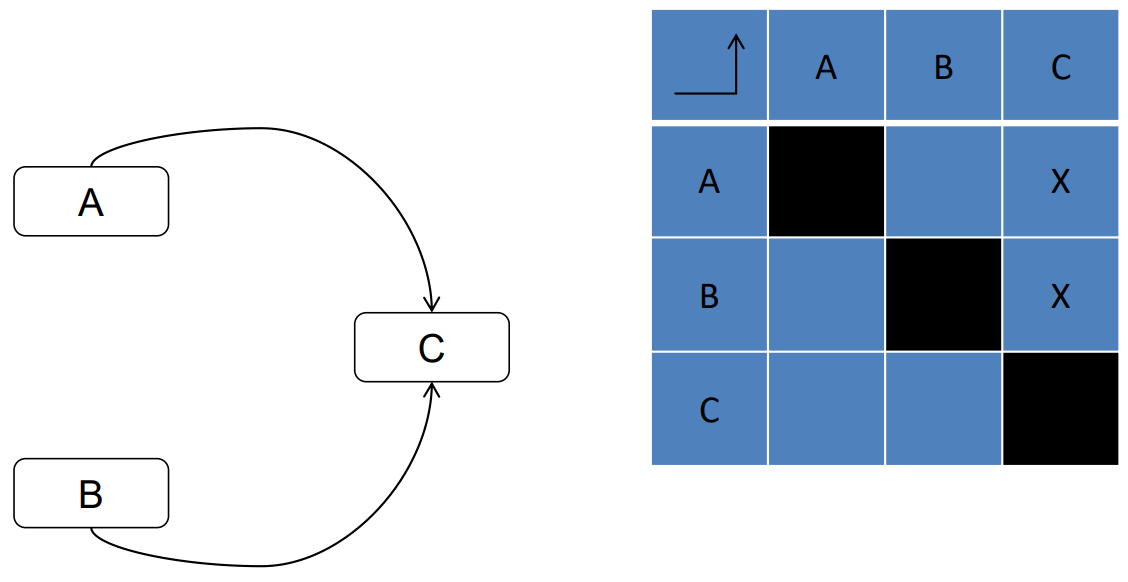
\includegraphics[width=0.6\linewidth]{Bilder/Teil3_MatrixRepresentationGerichtet.png}
    \caption{Beispiel Matrix Representation gerichteter Graph}
\end{figure}


% subsection
%-------------------------------------------------------------------------------------------
\subsection{Welche Arten von DSM gibt es?}

\begin{itemize}
    \item \textbf{Komponentenbasiert}
        \begin{itemize}
            \item Verbindungen von Komponenten.
            \item Anwendung in Systemarchitektur, Systems Engineering und System Design.
            \begin{figure}[H]
                \centering
                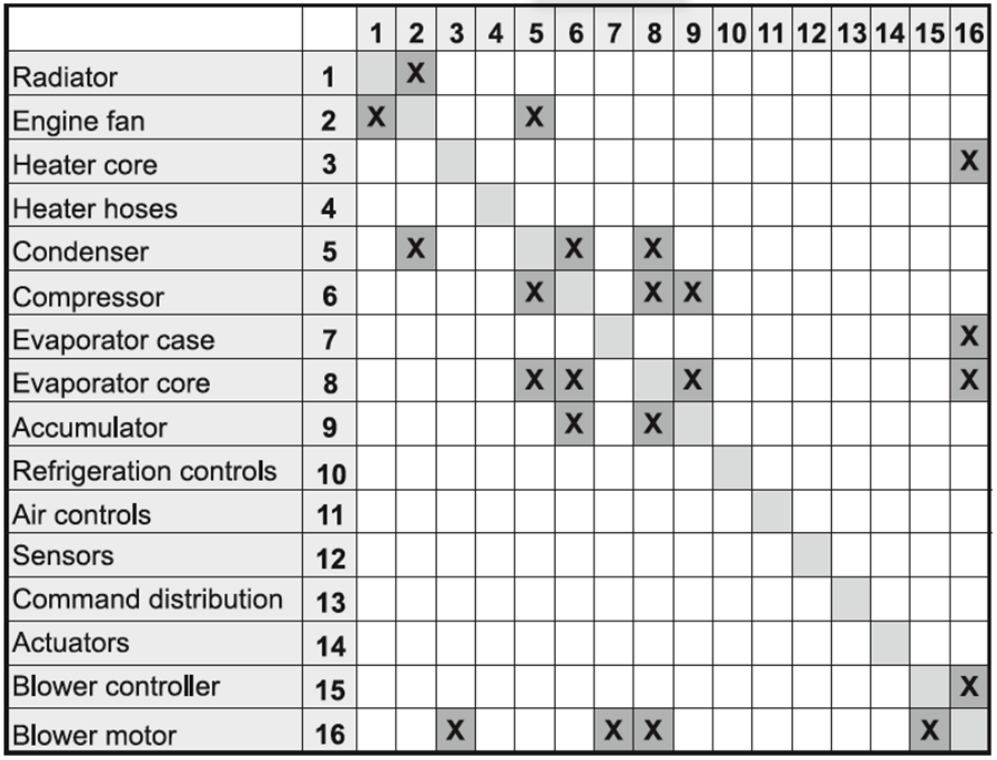
\includegraphics[width=0.6\linewidth]{Bilder/Teil3_KomponentenbasierteDSM.png}
                \caption{Komponentenbasierte DSM - Beispiel}
            \end{figure}
        \end{itemize}
    \item \textbf{Personenbasiert}
        \begin{itemize}
            \item Verbindung von Organisationseinheiten.
            \item Organisationsentwurf, Kommunikationsmanagement und Teamintegration.
            \begin{figure}[H]
                \centering
                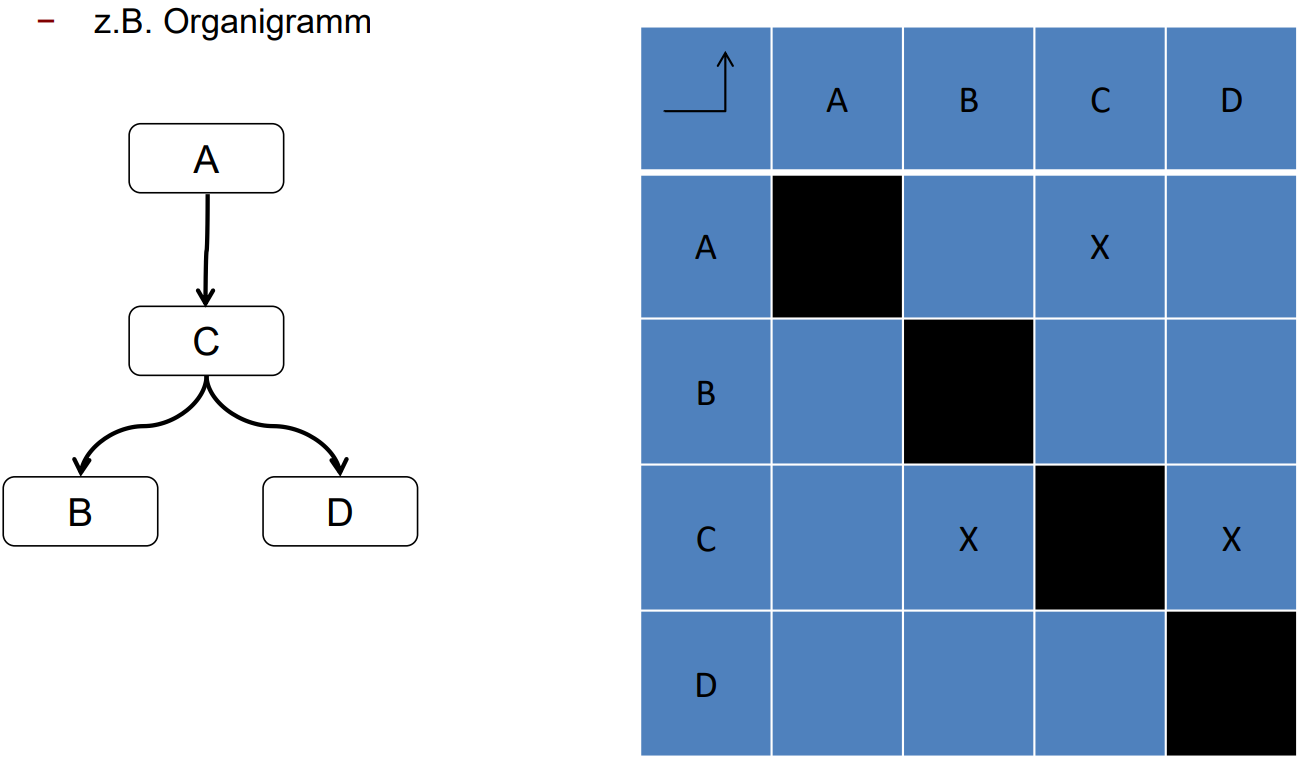
\includegraphics[width=0.6\linewidth]{Bilder/Teil3_PersonenbasierteDSM.png}
                \caption{Personenbasierte DSM - Beispiel}
            \end{figure}
        \end{itemize}
    \item \textbf{Aktivitätsbasiert}
        \begin{itemize}
            \item Verbindungen von Aktivitäten (Input / Output).
            \item Prozessverbesserung, Projektzeitplanung, Iterationsmanagement und Informationsflussmanagement.
            \begin{figure}[H]
                \centering
                \includegraphics[width=0.6\linewidth]{Bilder/Teil3_Aktivitätsbasierte DSM.png}
                \caption{Aktivitätenbasierte DSM - Beispiel}
            \end{figure}
        \end{itemize}
    \item \textbf{Parameterbasiert}
        \begin{itemize}
            \item Verbindungen von Design-Parametern.
            \item Aktivitätsabfolgen und Prozessentwurf.
            \begin{figure}[H]
                \centering
                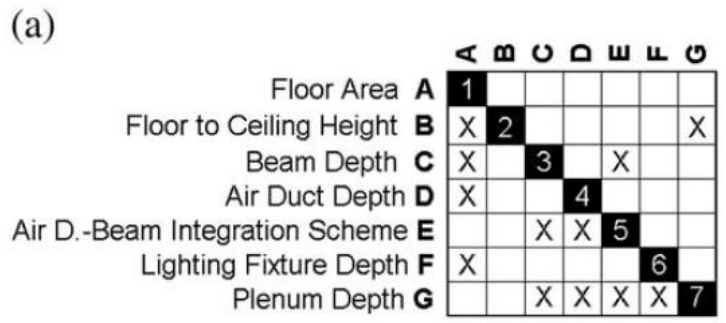
\includegraphics[width=0.6\linewidth]{Bilder/Teil3_ParameterbasierteDSM.png}
                \caption{Parameterbasierte DSM - Beispiel}
            \end{figure}
        \end{itemize}
\end{itemize}


% subsection
%-------------------------------------------------------------------------------------------
\subsection{Was bedeutet Sequenzierung von DSM?}

Sequenzierung ist die Umordnung der Zeilen und Spalten der DSM mit dem Ziel, dass es keine Schleifen gibt (Dreiecksmatrix).

\begin{itemize}
    \item Identifikation der Elemente ohne Information anderer Elemente ausgeführt werden könne.
        \\ Werden \textbf{nach links geschoben.}
    \item Identifikation die keine Information für andere Elemente liefert (Gegenteil von Punkt 1).
        \\ Werden \textbf{nach rechts geschoben.}
    \item Wenn Matrix nicht leer ist existiert mindestens eine Schleife. 
        \\ \textbf{Identifikations-Methoden:}
        \begin{itemize}
            \item Pfad Suchen.
            \item Adjazent Matrix.
            \item Erreichbarkeits Matrix Methode.
            \item Triangulations Algorithmus.
            \item Algorithms von Tarjan zur Bestimmung eines minimalen Spannungsbaumes.
        \end{itemize}
    \item \textbf{Beispiel einer Sequenzierung:}
        \begin{figure}[H]
            \centering
            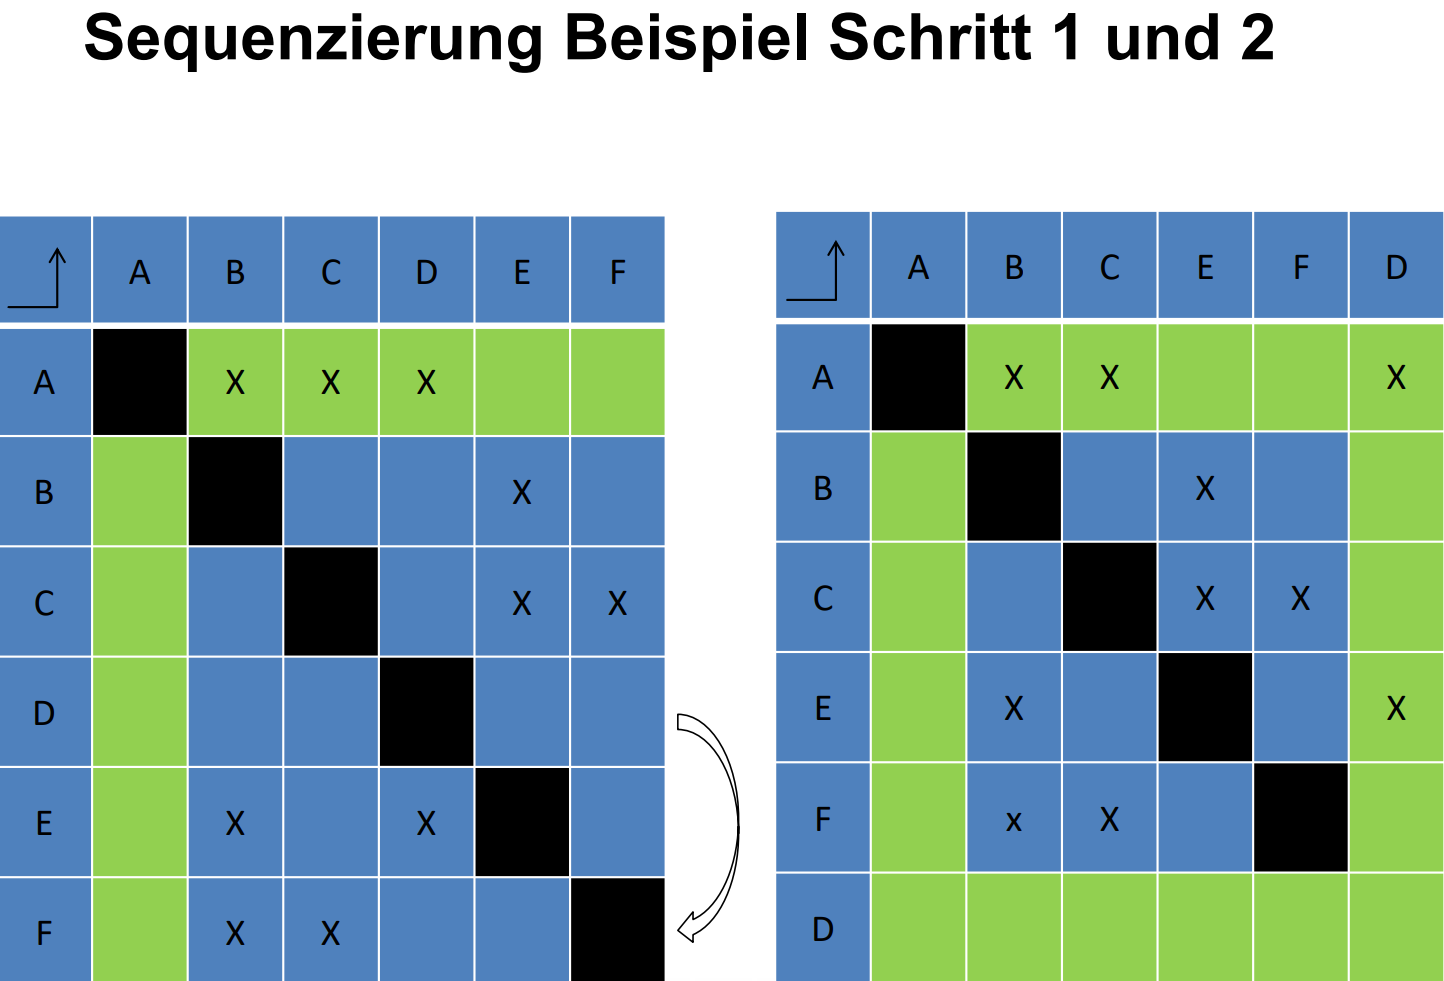
\includegraphics[width=0.8\linewidth]{Bilder/Teil3_SequenzierungBeispiel1.png}
            \caption{Sequenzierung Schritt 1 und 2 - Beispiel}
        \end{figure}
        \begin{figure}[H]
            \centering
            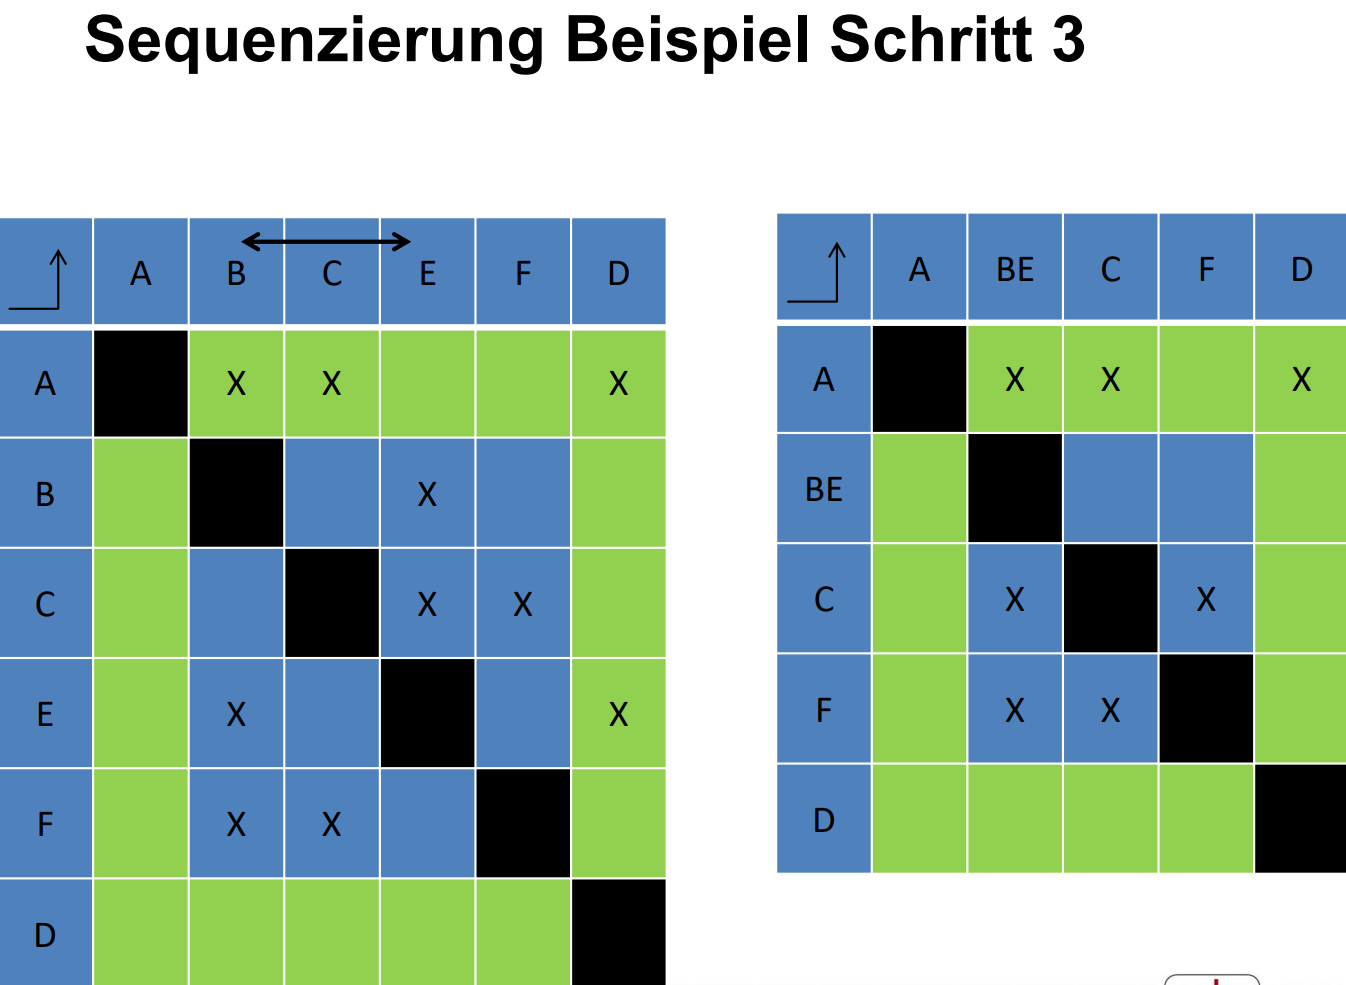
\includegraphics[width=0.8\linewidth]{Bilder/Teil3_SequenzierungBeispiel2.png}
            \caption{Sequenzierung Schritt 3 - Beispiel}
        \end{figure}
        \begin{figure}[H]
            \centering
            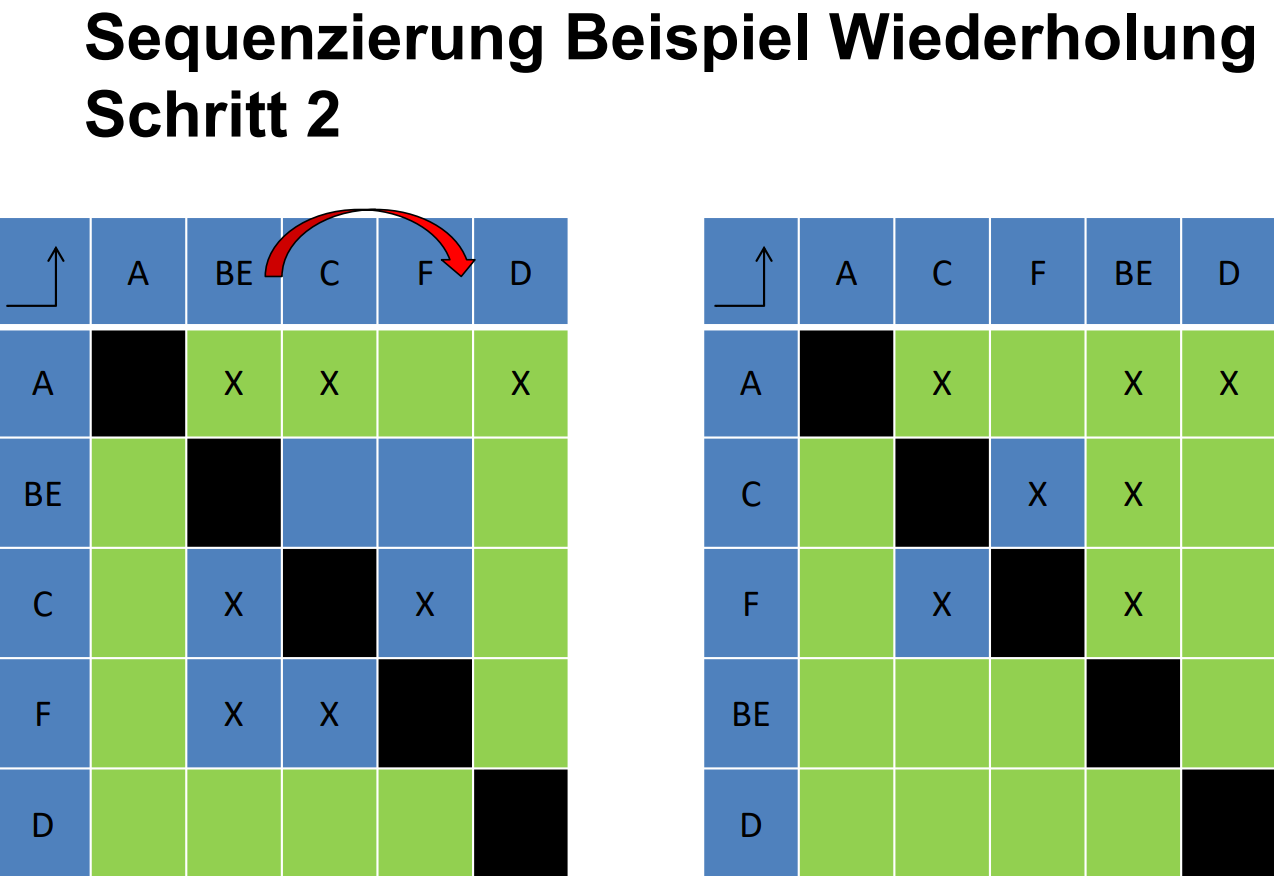
\includegraphics[width=0.8\linewidth]{Bilder/Teil3_SequenzierungBeispiel3.png}
            \caption{Sequenzierung Wiederholung Schritt 2 - Beispiel}
        \end{figure}
        \begin{figure}[H]
            \centering
            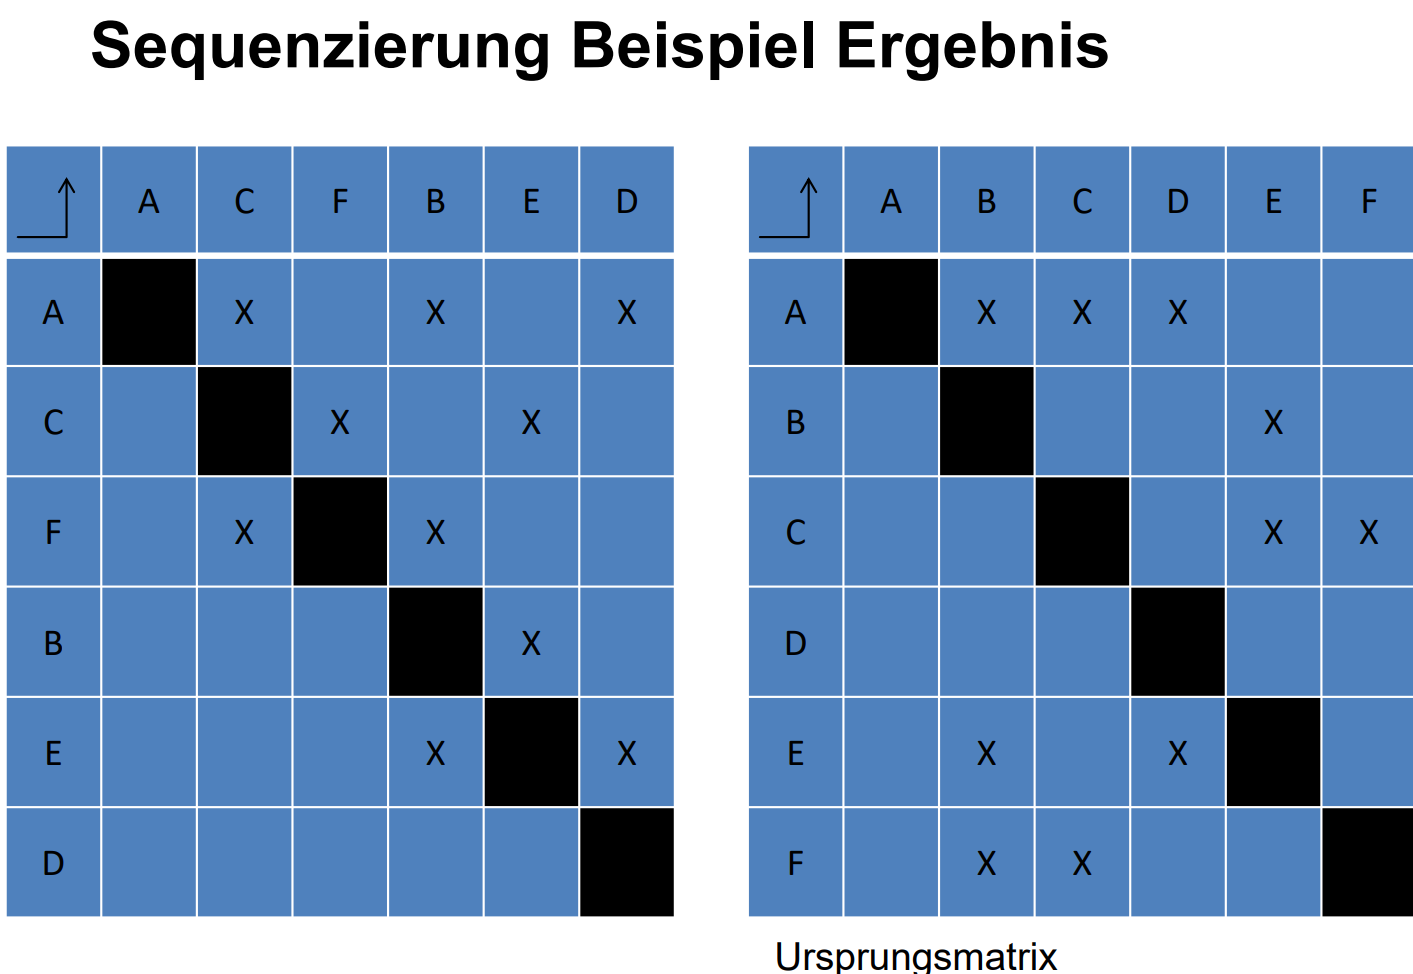
\includegraphics[width=0.8\linewidth]{Bilder/Teil3_SequenzierungBeispiel4.png}
            \caption{Sequenzierung Ergebnis - Beispiel}
        \end{figure}

        
\end{itemize}

% subsection
%-------------------------------------------------------------------------------------------
\subsection{Was bedeutet Clustering von DSM?}

Ziel ist es bei der Komponenten- bzw. Personenbasierten DSM \textbf{Cluster oder Module} zu identifizieren, in denen ein \textbf{Großteil der Interaktionen} stattfinden.

Clustering ermöglicht bessere Einblicke in die Teamorganisation und \textbf{Identifikation von Schlüsselparameter}.

\begin{figure}[H]
    \centering
    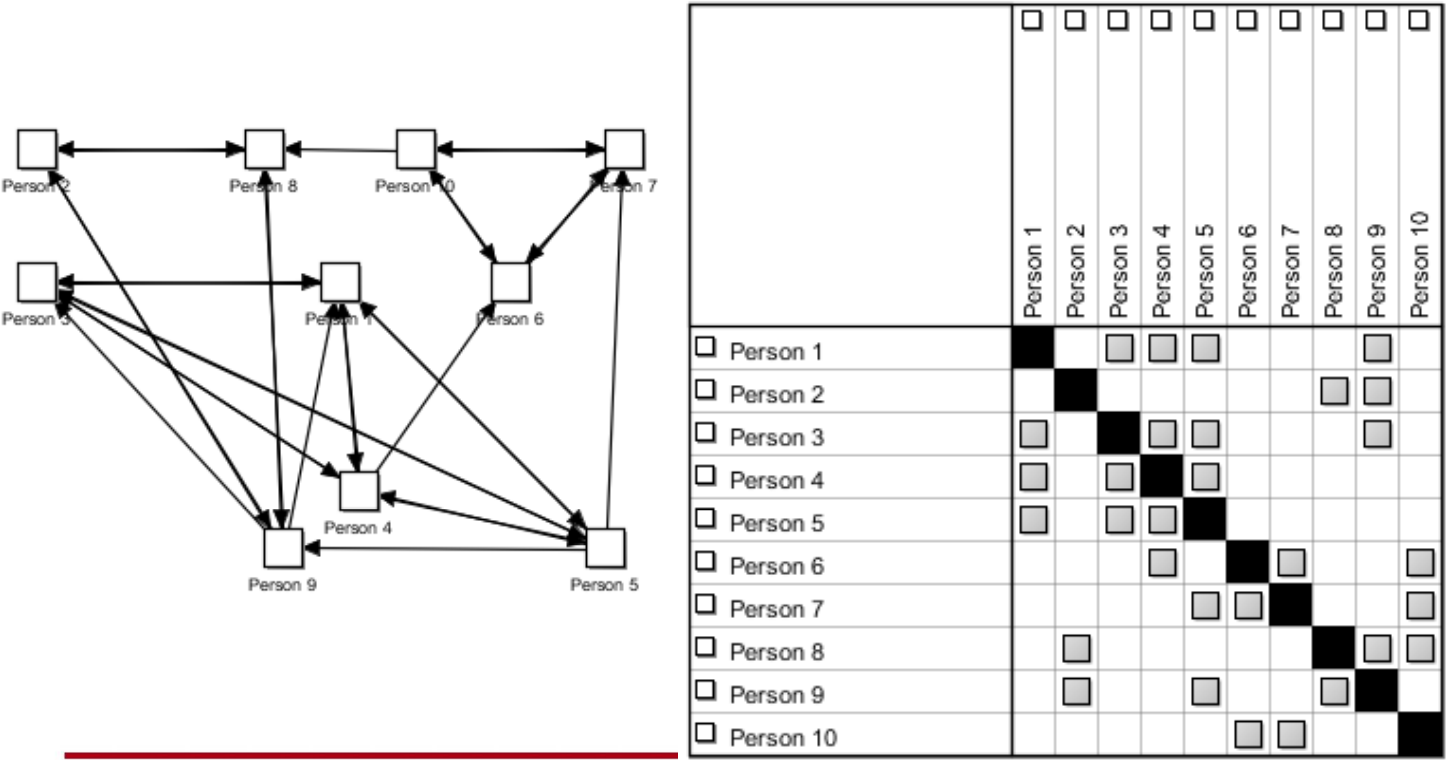
\includegraphics[width=0.8\linewidth]{Bilder/Teil3_ClusteringBeispiel.png}
    \caption{Clusterung - Beispiel}
\end{figure}



% Teil 4
\section{Teil}
beinhaltet folgende Foliensätze:

\begin{itemize}
    \item Teil 4:  Systemverhalten (Grundlagen der Modellplanung und –Bildung und Simulation)

\end{itemize}

% subsection
%-------------------------------------------------------------------------------------------
\subsection{Was ist ein Modell?}
Modelle sind Abstraktionen und Vereinfachung der Realität und zeigen deshalb nur Teilaspekte auf.
Es ist daher wichtig, dass die Modelle im Hinblick auf die Situation und die Problemstellung aussagekräftig sind.
Dies bedeutet, dass bei allen Überlegungen die Frage nach der Zweckmäßigkeit und der Problemrelevanz zu stellen ist.
\begin{figure}[H]
    \centering
    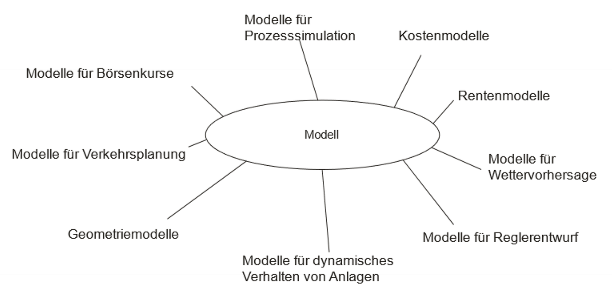
\includegraphics[width=0.6\linewidth]{Bilder/Teil4_ModelleBeispiel1.png}
    \caption{Beispiel Modelle verschiedener Lebensbereiche}
\end{figure}
% subsection
%-------------------------------------------------------------------------------------------
\subsection{Was bedeutet Problemlösung durch Abstraktion (Modellbildung) und Interpretation?}
Vorgehensweise der Modellbildung wird auf eine abstrakte Ebene verlagert, um die Lösungsfindung zu vereinfachen. 

\textbf{Zielgerichtete Vereinfachung durch Abstraktion.}

\begin{figure}[H]
    \centering
    \includegraphics[width=0.6\linewidth]{Bilder/Teil4_ProblemlösungdurchAbstraktionundInerpretation.png}
    \caption{Problemlösung durch Abstraktion und Interpretation}
\end{figure}

% subsection
%-------------------------------------------------------------------------------------------
\newpage
\subsection{Welche Verfahren der Modellbildung gibt es?}
\begin{itemize}
    \item \textbf{Rechnerische Verfahren:}\\
    Dazu werden \textbf{mathematische Modelle} benötigt, die formal durch \textbf{Gleichungen} beschrieben werden.
    
    Heutzutage stehen neben den traditionellen Methoden numerische und symbolische Softwareprogramme zu Verfügung.
    
    \item \textbf{Experimentelle bzw. messtechnische Verfahren:}\\
    Zu ihrer Anwendung werden \textbf{physikalische (experimentelle) Modelle} benötigt, an denen Versuche, Messungen und Auswertungen
    durchgeführt werden können. Dadurch sollen wesentliche Einflüsse messtechnisch erfasst werden.
    
    Im Maschinenbau etwa sind dies typischerweise Prototypen, Testobjekte, Versuchsanordnungen oder
    maßstäbliche Modelle.

    \item \textbf{Hybride Verfahren} (Kombination von Berechnung und Experiment bzw. Messung):\\
    Diese Verfahren \textbf{nutzen sowohl Messgrößen as auch mathematische Modelle.} Während bei rechnerischen Verfahren Fehler aufgrund
    von Modellierungsungenauigkeiten auftreten, sind bei experimentellen Verfahren mehr oder weniger große Messfehler unvermeidbar.
    
    Liegen sowohl mathematische Modelle als auch Messergebnisse vor, so kann man versuchen, Hypothesen über die Art der Fehler 
    zu bilden und das Modell anhand der Messergebnisse zu verbessern.
\end{itemize}

% subsection
%-------------------------------------------------------------------------------------------
\subsection{Wie ist der Ablauf zur Entstehung eines rechnerinternen Modells?}
\begin{itemize}
    \item Der Modellbildner entwickelt eine gedankliche Vorstellung des zu untersuchenden Originals (z.B. reales
    objekt oder neues Produkt) in Form eines mentalen Modells (Gedankenmodells), das anschließend 
    zu seiner Erfassung in eine formalisierte Informationsform mit Hilfe von Informationselementen und -strukturen gebracht wird.
    \item Dieses \glqq Informationsmodell\grqq wird am Rechner implementiert (rechnerinternes Modell).
\end{itemize}
\begin{figure}[H]
    \centering
    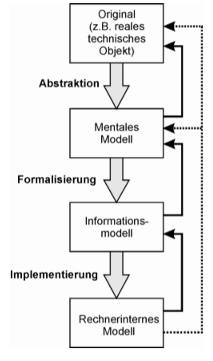
\includegraphics[width=0.3\linewidth]{Bilder/Teil4_RechnerinternesModell.png}
    \caption{Ablauf zur Entstehung eines rechnerinternen Modells}
\end{figure}

% subsection
%-------------------------------------------------------------------------------------------
\subsection{Was ist bei der Interpretation von Ergebnissen wichtig?}
Eine wichtige Aufgabe des Produktentwicklers ist die 
Interpretation der Ergebnisse. Dazu muss er zwischen physikalischen Phänomenen und künstlichen Effekten 
(Artefakten), die z.B. von Messfehlern bzw. numerischen Lösungsverfahren herrühren, unterscheiden können. 

Dies erfordert Kenntnisse und Erfahrung sowohl über die untersuchten Fragestellungen als auch über die Verfahren, die zur Lösung des Modellproblems verwendet werden. 

Einfache, überschlägige Abschätzungen und Erfahrung sind unerlässlich, um die Ergebnisse (Messergebnisse bzw. Rechenergebnisse) 
zu überprüfen sowie zu bewerten und damit hohe Qualität der Simulation sicherzustellen.

% subsection
%-------------------------------------------------------------------------------------------
\subsection{Was bedeutet Simulation und wofür ist dies relevant?}

Simulation ist ein Verfahren zur Nachbildung eines Systems mit seinen 
dynamischen Prozessen in einem experimentierbaren Modell, um zu 
Erkenntnissen zu gelangen, die auf die Wirklichkeit übertragbar sind. 

Im weiteren Sinne wird unter Simulation das Vorbereiten, Durchführen und 
Auswerten gezielter Experimente mit einem Simulationsmodell verstanden. 

Mit Hilfe der Simulation kann das zeitliche Ablaufverhalten komplexer Systeme 
untersucht werden.    

Simulationen werden durchgeführt wenn:
\begin{itemize}
    \item kein reales System verfügbar ist (Entwurfsphase)
    \item das Experiment am realen System zu lange dauert
    \item das Experiment am realen System zu teuer ist
    \item das Experiment am realen System zu gefährlich ist (Flugzeug, Kraftwerk)
    \item die Zeitkonstanten des realen Systems zu groß sind (Klimamodelle)
\end{itemize}

% Teil 5
\section{Teil}
beinhaltet folgende Foliensätze:

\begin{itemize}
    \item Teil 5: Digitaler Zwilling

\end{itemize}

% subsection
%-------------------------------------------------------------------------------------------
\subsection{Erklären Sie in eigenen Worten den Begriff Digitaler Zwilling!}
Ein Digitaler Zwilling ist ein virtuelles Abbild eines realen Objekts oder Systems. 
Er besteht aus dem realen Objekt, dem digitalen Modell und den Daten, die beide miteinander verbinden, um das reale Objekt in Echtzeit oder für Simulationen abzubilden.


% subsection
%-------------------------------------------------------------------------------------------
\subsection{Was ist ein Digitaler Schatten?}
Ein Digitaler Schatten beschreibt die Echtzeitdarstellung von Betriebs-, Zustands- oder Prozessdaten eines realen Objekts oder Systems, ohne dass ein vollständiges Modell vorliegt. 
Er wird durch die Daten aus der realen Welt generiert.\\
\\
Ein Digitaler Schatten ist eine Echtzeitdarstellung der Betriebs- oder Prozessdaten eines realen Objekts oder Systems. 
Im Gegensatz zum Digitalen Zwilling umfasst er kein vollständiges Modell, sondern nur die kontinuierlich erfassten Daten, die den aktuellen Zustand des Systems widerspiegeln. 
Diese Daten ermöglichen die Überwachung und Analyse des realen Objekts ohne Modellierung des gesamten Verhaltens.


% subsection
%-------------------------------------------------------------------------------------------
\subsection{Was bedeutet Functional Mock-Up Interface?}
Das Functional Mock-Up Interface (FMI) ist eine standardisierte Schnittstelle, die den Austausch und die Integration von Simulationsmodellen zwischen verschiedenen Softwareumgebungen ermöglicht. 
Es erlaubt die Kosimulation, bei der Modelle in verschiedenen Tools gemeinsam ausgeführt werden, ohne dass das Modell in jedem Tool neu erstellt werden muss.

\end{document}




%-------------------------------------------------------------------------------------------
\begin{comment}
------------------------------------------------------------------------------------------------
Mögliche Zusätze:

Teil 2:
Anforderungen Validierung vs Verifikation
Anforderungen verwalten

Teil3:
Produktstruktur (Bereiche, Freiheitsgrade)
DSM Lesekonvektion
Weitere DSM (Vor Arten DSM)
klassifizierung DSM
Erstellen / Aufbauen DSM












---------------------------------------------------------------------------------------------
Bereich für Code Vorlagen für Copy-Paste:


---Einfache Aufzählung---

\begin{itemize}
    \item Erster
    \item Zweiter
    \item Dritter
\end{itemize}


---Aufzählung mit Beschreibung---

\begin{description}[style=nextline]
    \item[Begriff1] Beschreibung1
    \item[Begriff2] Beschreibung2
    \item[Begriff3] Beschreibung3
\end{description}

itemsep=0pt: Abstand zwischen den einzelnen Listenelementen.
topsep=0pt: vertikalen Abstand vor und nach der gesamten Liste.
parsep=0pt: Abstand zwischen Absätzen innerhalb der Listenelemente.
partopsep=0pt: Abstand zwischen den Listenelementen und dem vorherigen oder folgenden Text.

---Aufzählung mit Unterpunkten---

\begin{itemize}
    \item ErsterPunkt
        \begin{itemize}
            \item Unterpunkt1
            \item Unterpunkt2
        \end{itemize}
    \item ZweiterPunkt
        \begin{itemize}
            \item Unterpunkt1
            \item Unterpunkt2
        \end{itemize}
\end{itemize}


---Einzelnes Bild---

\begin{figure}[H]
    \centering
    \includegraphics[width=0.8\linewidth]{Pfad}
    \caption{CAPTION}
    \label{LABEL}
\end{figure}

---Zwei Bilder nebeneinander---

\begin{figure}[H]
    \centering
    \begin{minipage}[t]{0.45\textwidth}  % 't' sorgt dafür, dass die minipage an der Oberkante ausgerichtet ist
        \centering
        \includegraphics[width=\linewidth]{Pfad1}
        \caption{Caption1}
    \end{minipage} \hfill
    \begin{minipage}[t]{0.45\textwidth}  % 't' sorgt für gleiche Ausrichtung der Unterschriften
        \centering
        \includegraphics[width=\linewidth]{Pfad2}
        \caption{Caption2}
    \end{minipage}
    \caption{CaptionBeide}
\end{figure}

\end{comment}